
%% bare_jrnl_transmag.tex
%% V1.4a
%% 2014/09/17
%% by Michael Shell
%% see http://www.michaelshell.org/
%% for current contact information.
%%
%% This is a skeleton file demonstrating the use of IEEEtran.cls
%% (requires IEEEtran.cls version 1.8a or later) with an IEEE 
%% Transactions on Magnetics journal paper.
%%
%% Support sites:
%% http://www.michaelshell.org/tex/ieeetran/
%% http://www.ctan.org/tex-archive/macros/latex/contrib/IEEEtran/
%% and
%% http://www.ieee.org/

%%*************************************************************************
%% Legal Notice:
%% This code is offered as-is without any warranty either expressed or
%% implied; without even the implied warranty of MERCHANTABILITY or
%% FITNESS FOR A PARTICULAR PURPOSE! 
%% User assumes all risk.
%% In no event shall IEEE or any contributor to this code be liable for
%% any damages or losses, including, but not limited to, incidental,
%% consequential, or any other damages, resulting from the use or misuse
%% of any information contained here.
%%
%% All comments are the opinions of their respective authors and are not
%% necessarily endorsed by the IEEE.
%%
%% This work is distributed under the LaTeX Project Public License (LPPL)
%% ( http://www.latex-project.org/ ) version 1.3, and may be freely used,
%% distributed and modified. A copy of the LPPL, version 1.3, is included
%% in the base LaTeX documentation of all distributions of LaTeX released
%% 2003/12/01 or later.
%% Retain all contribution notices and credits.
%% ** Modified files should be clearly indicated as such, including  **
%% ** renaming them and changing author support contact information. **
%%
%% File list of work: IEEEtran.cls, IEEEtran_HOWTO.pdf, bare_adv.tex,
%%                    bare_conf.tex, bare_jrnl.tex, bare_conf_compsoc.tex,
%%                    bare_jrnl_compsoc.tex, bare_jrnl_transmag.tex
%%*************************************************************************


% *** Authors should verify (and, if needed, correct) their LaTeX system  ***
% *** with the testflow diagnostic prior to trusting their LaTeX platform ***
% *** with production work. IEEE's font choices and paper sizes can       ***
% *** trigger bugs that do not appear when using other class files.       ***                          ***
% The testflow support page is at:
% http://www.michaelshell.org/tex/testflow/



\documentclass[journal,transmag,twoside]{IEEEtran}
%
% If IEEEtran.cls has not been installed into the LaTeX system files,
% manually specify the path to it like:
% \documentclass[journal]{../sty/IEEEtran}





% Some very useful LaTeX packages include:
% (uncomment the ones you want to load)


% *** MISC UTILITY PACKAGES ***
%
%\usepackage{ifpdf}
% Heiko Oberdiek's ifpdf.sty is very useful if you need conditional
% compilation based on whether the output is pdf or dvi.
% usage:
% \ifpdf
%   % pdf code
% \else
%   % dvi code
% \fi
% The latest version of ifpdf.sty can be obtained from:
% http://www.ctan.org/tex-archive/macros/latex/contrib/oberdiek/
% Also, note that IEEEtran.cls V1.7 and later provides a builtin
% \ifCLASSINFOpdf conditional that works the same way.
% When switching from latex to pdflatex and vice-versa, the compiler may
% have to be run twice to clear warning/error messages.






% *** CITATION PACKAGES ***
%
%\usepackage{cite}
% cite.sty was written by Donald Arseneau
% V1.6 and later of IEEEtran pre-defines the format of the cite.sty package
% \cite{} output to follow that of IEEE. Loading the cite package will
% result in citation numbers being automatically sorted and properly
% "compressed/ranged". e.g., [1], [9], [2], [7], [5], [6] without using
% cite.sty will become [1], [2], [5]--[7], [9] using cite.sty. cite.sty's
% \cite will automatically add leading space, if needed. Use cite.sty's
% noadjust option (cite.sty V3.8 and later) if you want to turn this off
% such as if a citation ever needs to be enclosed in parenthesis.
% cite.sty is already installed on most LaTeX systems. Be sure and use
% version 5.0 (2009-03-20) and later if using hyperref.sty.
% The latest version can be obtained at:
% http://www.ctan.org/tex-archive/macros/latex/contrib/cite/
% The documentation is contained in the cite.sty file itself.






% *** GRAPHICS RELATED PACKAGES ***
%
\ifCLASSINFOpdf
  \usepackage[pdftex]{graphicx}
  % declare the path(s) where your graphic files are
  % \graphicspath{{../pdf/}{../jpeg/}}
  % and their extensions so you won't have to specify these with
  % every instance of \includegraphics
  % \DeclareGraphicsExtensions{.pdf,.jpeg,.png}
\else
  % or other class option (dvipsone, dvipdf, if not using dvips). graphicx
  % will default to the driver specified in the system graphics.cfg if no
  % driver is specified.
  % \usepackage[dvips]{graphicx}
  % declare the path(s) where your graphic files are
  % \graphicspath{{../eps/}}
  % and their extensions so you won't have to specify these with
  % every instance of \includegraphics
  % \DeclareGraphicsExtensions{.eps}
\fi
% graphicx was written by David Carlisle and Sebastian Rahtz. It is
% required if you want graphics, photos, etc. graphicx.sty is already
% installed on most LaTeX systems. The latest version and documentation
% can be obtained at: 
% http://www.ctan.org/tex-archive/macros/latex/required/graphics/
% Another good source of documentation is "Using Imported Graphics in
% LaTeX2e" by Keith Reckdahl which can be found at:
% http://www.ctan.org/tex-archive/info/epslatex/
%
% latex, and pdflatex in dvi mode, support graphics in encapsulated
% postscript (.eps) format. pdflatex in pdf mode supports graphics
% in .pdf, .jpeg, .png and .mps (metapost) formats. Users should ensure
% that all non-photo figures use a vector format (.eps, .pdf, .mps) and
% not a bitmapped formats (.jpeg, .png). IEEE frowns on bitmapped formats
% which can result in "jaggedy"/blurry rendering of lines and letters as
% well as large increases in file sizes.
%
% You can find documentation about the pdfTeX application at:
% http://www.tug.org/applications/pdftex




% *** MATH PACKAGES ***
%
%\usepackage[cmex10]{amsmath}
% A popular package from the American Mathematical Society that provides
% many useful and powerful commands for dealing with mathematics. If using
% it, be sure to load this package with the cmex10 option to ensure that
% only type 1 fonts will utilized at all point sizes. Without this option,
% it is possible that some math symbols, particularly those within
% footnotes, will be rendered in bitmap form which will result in a
% document that can not be IEEE Xplore compliant!
%
% Also, note that the amsmath package sets \interdisplaylinepenalty to 10000
% thus preventing page breaks from occurring within multiline equations. Use:
%\interdisplaylinepenalty=2500
% after loading amsmath to restore such page breaks as IEEEtran.cls normally
% does. amsmath.sty is already installed on most LaTeX systems. The latest
% version and documentation can be obtained at:
% http://www.ctan.org/tex-archive/macros/latex/required/amslatex/math/





% *** SPECIALIZED LIST PACKAGES ***
%
%\usepackage{algorithmic}
% algorithmic.sty was written by Peter Williams and Rogerio Brito.
% This package provides an algorithmic environment fo describing algorithms.
% You can use the algorithmic environment in-text or within a figure
% environment to provide for a floating algorithm. Do NOT use the algorithm
% floating environment provided by algorithm.sty (by the same authors) or
% algorithm2e.sty (by Christophe Fiorio) as IEEE does not use dedicated
% algorithm float types and packages that provide these will not provide
% correct IEEE style captions. The latest version and documentation of
% algorithmic.sty can be obtained at:
% http://www.ctan.org/tex-archive/macros/latex/contrib/algorithms/
% There is also a support site at:
% http://algorithms.berlios.de/index.html
% Also of interest may be the (relatively newer and more customizable)
% algorithmicx.sty package by Szasz Janos:
% http://www.ctan.org/tex-archive/macros/latex/contrib/algorithmicx/




% *** ALIGNMENT PACKAGES ***
%
%\usepackage{array}
% Frank Mittelbach's and David Carlisle's array.sty patches and improves
% the standard LaTeX2e array and tabular environments to provide better
% appearance and additional user controls. As the default LaTeX2e table
% generation code is lacking to the point of almost being broken with
% respect to the quality of the end results, all users are strongly
% advised to use an enhanced (at the very least that provided by array.sty)
% set of table tools. array.sty is already installed on most systems. The
% latest version and documentation can be obtained at:
% http://www.ctan.org/tex-archive/macros/latex/required/tools/


% IEEEtran contains the IEEEeqnarray family of commands that can be used to
% generate multiline equations as well as matrices, tables, etc., of high
% quality.




% *** SUBFIGURE PACKAGES ***
%\ifCLASSOPTIONcompsoc
%  \usepackage[caption=false,font=normalsize,labelfont=sf,textfont=sf]{subfig}
%\else
%  \usepackage[caption=false,font=footnotesize]{subfig}
%\fi
% subfig.sty, written by Steven Douglas Cochran, is the modern replacement
% for subfigure.sty, the latter of which is no longer maintained and is
% incompatible with some LaTeX packages including fixltx2e. However,
% subfig.sty requires and automatically loads Axel Sommerfeldt's caption.sty
% which will override IEEEtran.cls' handling of captions and this will result
% in non-IEEE style figure/table captions. To prevent this problem, be sure
% and invoke subfig.sty's "caption=false" package option (available since
% subfig.sty version 1.3, 2005/06/28) as this is will preserve IEEEtran.cls
% handling of captions.
% Note that the Computer Society format requires a larger sans serif font
% than the serif footnote size font used in traditional IEEE formatting
% and thus the need to invoke different subfig.sty package options depending
% on whether compsoc mode has been enabled.
%
% The latest version and documentation of subfig.sty can be obtained at:
% http://www.ctan.org/tex-archive/macros/latex/contrib/subfig/



% *** FLOAT PACKAGES ***
%
%\usepackage{fixltx2e}
% fixltx2e, the successor to the earlier fix2col.sty, was written by
% Frank Mittelbach and David Carlisle. This package corrects a few problems
% in the LaTeX2e kernel, the most notable of which is that in current
% LaTeX2e releases, the ordering of single and double column floats is not
% guaranteed to be preserved. Thus, an unpatched LaTeX2e can allow a
% single column figure to be placed prior to an earlier double column
% figure. The latest version and documentation can be found at:
% http://www.ctan.org/tex-archive/macros/latex/base/


%\usepackage{stfloats}
% stfloats.sty was written by Sigitas Tolusis. This package gives LaTeX2e
% the ability to do double column floats at the bottom of the page as well
% as the top. (e.g., "\begin{figure*}[!b]" is not normally possible in
% LaTeX2e). It also provides a command:
%\fnbelowfloat
% to enable the placement of footnotes below bottom floats (the standard
% LaTeX2e kernel puts them above bottom floats). This is an invasive package
% which rewrites many portions of the LaTeX2e float routines. It may not work
% with other packages that modify the LaTeX2e float routines. The latest
% version and documentation can be obtained at:
% http://www.ctan.org/tex-archive/macros/latex/contrib/sttools/
% Do not use the stfloats baselinefloat ability as IEEE does not allow
% \baselineskip to stretch. Authors submitting work to the IEEE should note
% that IEEE rarely uses double column equations and that authors should try
% to avoid such use. Do not be tempted to use the cuted.sty or midfloat.sty
% packages (also by Sigitas Tolusis) as IEEE does not format its papers in
% such ways.
% Do not attempt to use stfloats with fixltx2e as they are incompatible.
% Instead, use Morten Hogholm'a dblfloatfix which combines the features
% of both fixltx2e and stfloats:
%
% \usepackage{dblfloatfix}
% The latest version can be found at:
% http://www.ctan.org/tex-archive/macros/latex/contrib/dblfloatfix/




%\ifCLASSOPTIONcaptionsoff
%  \usepackage[nomarkers]{endfloat}
% \let\MYoriglatexcaption\caption
% \renewcommand{\caption}[2][\relax]{\MYoriglatexcaption[#2]{#2}}
%\fi
% endfloat.sty was written by James Darrell McCauley, Jeff Goldberg and 
% Axel Sommerfeldt. This package may be useful when used in conjunction with 
% IEEEtran.cls'  captionsoff option. Some IEEE journals/societies require that
% submissions have lists of figures/tables at the end of the paper and that
% figures/tables without any captions are placed on a page by themselves at
% the end of the document. If needed, the draftcls IEEEtran class option or
% \CLASSINPUTbaselinestretch interface can be used to increase the line
% spacing as well. Be sure and use the nomarkers option of endfloat to
% prevent endfloat from "marking" where the figures would have been placed
% in the text. The two hack lines of code above are a slight modification of
% that suggested by in the endfloat docs (section 8.4.1) to ensure that
% the full captions always appear in the list of figures/tables - even if
% the user used the short optional argument of \caption[]{}.
% IEEE papers do not typically make use of \caption[]'s optional argument,
% so this should not be an issue. A similar trick can be used to disable
% captions of packages such as subfig.sty that lack options to turn off
% the subcaptions:
% For subfig.sty:
% \let\MYorigsubfloat\subfloat
% \renewcommand{\subfloat}[2][\relax]{\MYorigsubfloat[]{#2}}
% However, the above trick will not work if both optional arguments of
% the \subfloat command are used. Furthermore, there needs to be a
% description of each subfigure *somewhere* and endfloat does not add
% subfigure captions to its list of figures. Thus, the best approach is to
% avoid the use of subfigure captions (many IEEE journals avoid them anyway)
% and instead reference/explain all the subfigures within the main caption.
% The latest version of endfloat.sty and its documentation can obtained at:
% http://www.ctan.org/tex-archive/macros/latex/contrib/endfloat/
%
% The IEEEtran \ifCLASSOPTIONcaptionsoff conditional can also be used
% later in the document, say, to conditionally put the References on a 
% page by themselves.




% *** PDF, URL AND HYPERLINK PACKAGES ***
%
\usepackage{url}
% url.sty was written by Donald Arseneau. It provides better support for
% handling and breaking URLs. url.sty is already installed on most LaTeX
% systems. The latest version and documentation can be obtained at:
% http://www.ctan.org/tex-archive/macros/latex/contrib/url/
% Basically, \url{my_url_here}.

\usepackage{hyperref}
\newcommand{\email}[1]{\href{mailto:#1}{#1}}

\usepackage{pdfcomment}
\usepackage{xcolor}
\newcommand{\karrcomment}[2]{\pdfmarkupcomment[markup=Highlight,color=yellow,author={Jonathan Karr}]{#1}{#2}}
\usepackage{pgfplots}
\usepackage{caption}
\usepackage{subcaption}
\usepackage{fancyvrb}

% *** Do not adjust lengths that control margins, column widths, etc. ***
% *** Do not use packages that alter fonts (such as pslatex).         ***
% There should be no need to do such things with IEEEtran.cls V1.6 and later.
% (Unless specifically asked to do so by the journal or conference you plan
% to submit to, of course. )

\usepackage{color,soul} % for highlighting only

%http://tex.stackexchange.com/questions/61265/why-doesnt-the-ieeetran-document-class-recognize-definition-environments
\newtheorem{definition}{Definition}

% correct bad hyphenation here
\hyphenation{op-tical net-works semi-conduc-tor}

% Nature News on irreproducibility:
% http://www.nature.com/news/reproducibility-1.17552

\begin{document}

\title{Engineering Dynamical Models for Better Reproducibility}

\author{
    J. Kyle Medley$^*$ and
	Jonathan R. Karr
    
    \thanks{
        Manuscript received XXX XX, 2015; revised XXX XX, 2016; accepted XXX XX, 2016. Date of publication XXX XX, 2016; date of current version XXX XX, 2016.
        J. K. Medley was supported by National Institutes of Health grant R01 GM081070. J. R. Karr was supported by National Science Foundation grant 1548123 and a James S. McDonnell Foundation Postdoctoral Fellowship Award in Studying Complex Systems. The content is solely the responsibility of the authors and does not necessarily represent the views of the National Institutes of Health, the National Science Foundation, or the James S. McDonnell Foundation.
        \textit{Asterisk indicates corresponding author.}
    }
    \thanks{$^*$J. K. Medley is with the Department of Bioengineering, University of Washington, Seattle, WA 98195, USA (e-mail: \email{medleyj@uw.edu}).}
    \thanks{J. R. Karr is with the Department of Genetics \& Genomic Sciences, Icahn School of Medicine at Mount Sinai, New York, NY 10029, USA (e-mail: \email{karr@mssm.edu}).}
    \thanks{Digital Object Identifier 10.1109/TBME.XXXX.XXXXXXX}
}

% The paper headers
\markboth{IEEE Transactions on Biomedical Engineering,~Vol.~13, No.~9, October~2015}%
{Medley \MakeLowercase{\textit{et al.}}: Enginnering Dynamical Models for Better Reproducibility}
% The only time the second header will appear is for the odd numbered pages
% after the title page when using the twoside option.
% 
% *** Note that you probably will NOT want to include the author's ***
% *** name in the headers of peer review papers.                   ***
% You can use \ifCLASSOPTIONpeerreview for conditional compilation here if
% you desire.




% If you want to put a publisher's ID mark on the page you can do it like
% this:
%\IEEEpubid{0000--0000/00\$00.00~\copyright~2014 IEEE}
% Remember, if you use this you must call \IEEEpubidadjcol in the second
% column for its text to clear the IEEEpubid mark.



% use for special paper notices
%\IEEEspecialpapernotice{(Invited Paper)}

\maketitle

\begin{abstract}
\textit{Objective:} To outline the requirements for reproducible dynamical models in systems biology.
\textit{Methods:} We describe the standards and software tools that are needed to enable researchers to reproduce models and simulations.
\textit{Results:} We show that it is possible to engineer models and software tools for better reproducibility
by using deterministic algorithms, data integration, and explicit documentation of assumptions.
\textit{Conclusion:} While dynamical modeling has made great strides with the creation of the first whole-cell (WC) model of \textit{Mycoplasma genitalium},
continuing to advance dynamical modeling requires reproducing increasingly complex models and simulations.
Building an ecosystem of software and standards which emphasize reproducibility
is a necessary step in achieving this goal.
\textit{Significance:}
It is currently challenging to reproduce complex simulations. Here, we
suggest how future tools
and standards might be tailored to meet upcoming challenges in reproducible modeling.
We use WC modeling as an example throughout our discussion.
\end{abstract}

\begin{IEEEkeywords}
Systems biology, computational modeling, reproducibility
\end{IEEEkeywords}

% To allow for easy dual compilation without having to reenter the
% abstract/keywords data, the \IEEEtitleabstractindextext text will
% not be used in maketitle, but will appear (i.e., to be "transported")
% here as \IEEEdisplaynontitleabstractindextext when the compsoc 
% or transmag modes are not selected <OR> if conference mode is selected 
% - because all conference papers position the abstract like regular
% papers do.
\IEEEdisplaynontitleabstractindextext
% \IEEEdisplaynontitleabstractindextext has no effect when using
% compsoc or transmag under a non-conference mode.







% For peer review papers, you can put extra information on the cover
% page as needed:
% \ifCLASSOPTIONpeerreview
% \begin{center} \bfseries EDICS Category: 3-BBND \end{center}
% \fi
%
% For peerreview papers, this IEEEtran command inserts a page break and
% creates the second title. It will be ignored for other modes.
\IEEEpeerreviewmaketitle



\section{Introduction}
% The very first letter is a 2 line initial drop letter followed
% by the rest of the first word in caps.
% 
% form to use if the first word consists of a single letter:
% \IEEEPARstart{A}{demo} file is ....
% 
% form to use if you need the single drop letter followed by
% normal text (unknown if ever used by IEEE):
% \IEEEPARstart{A}{}demo file is ....
% 
% Some journals put the first two words in caps:
% \IEEEPARstart{T}{his demo} file is ....
% 
% Here we have the typical use of a "T" for an initial drop letter
% and "HIS" in caps to complete the first word.
\IEEEPARstart{R}{eproducibility} is one of the central tenets of the scientific method.
\textit{Reproducibility} is the ability to confirm a result via a completely independent test, including different investigators, experimental methods, and experimental machinery. 
This rigorous standard eliminates conclusions that were based on incorrect methods, machinery, or experiments and ensures that scientific results are only accepted as facts once multiple scientists have thoroughly dismissed other potential explanations. 

\textit{Repeatability}, in contrast, is the ability to reproduce a result given the same experimental machinery and conditions.
% Repeatability is a more liberal standard than reproducibility because replicability does not require independent experimental methods or equipment.
Consequently, replicability only has the power to eliminate conclusions that were based on erroneous experiments, and cannot eliminate conclusions based on faulty methods or machinery.

To illustrate the difference between these two terms, consider a Gedanken experiment where Alice is trying to \textit{reproduce} a result published by Bob concerning pathway X, which has been implicated in cancer. The pathway has several regulators and Bob's results predict that knocking out the ONCO1 regulator alone is sufficient to cause cancer. Alice's results contradict this. In fact, she finds that at least two or more regulators must be knocked out in order to cause cancer. Since Bob's simulation algorithm was published along with his results, Alice should in theory be able to download and run his simulations. Assume that Bob used a technology such as SED-ML \cite{sedml2011} to parameterize his model so that Alice knows unambiguously what parameter values he used to obtain his results. She initializes her model with the same values and finds that, at the initial state, most of the processes in her model have the same reaction rates as Bob's, except for the activity of ONCO1 and several other regulators. Further investigation confirms that the kinetic laws for these interactions are different, which she later traces back to a decoupling assumption in Bob's model.

The above example shows that \textit{reproducibility} applies to a process with a human in the loop. Different researchers are unlikely to arrive at the same numerical results, but tracking down discrepancies often helps illuminate sources of error. By contrast, machines can, in principle, replicate a numerical result exactly without human intervetion. \textit{Replicability} is a technological feature, whereas \textit{reproducibility} is a property of the research process.

In systems biology, many standards have been introduced for encoding models and simulations. These standards include CellML \cite{cuellar2003overview}, SBML \cite{hucka2003}, SED-ML \cite{sedml2011}, the COMBINE archive \cite{COMBINE2012}, and SBGN \cite{LeNovereHMMSS09} and model repositories including BioModels and the CellML Model Repository.
By utilizing community-based development \cite{hucka2015promoting} \cite{drager2014improving}, these standards are tailored to a wide range of use-cases in modeling and allow researchers to reproduce most \textit{in silico} experiments using a range of simulation tools. These standards and repositories have also enabled researchers to reuse models for new experiments, to expand models, and to combine models into larger, more comprehensive models. By encouraging reuse and modification of models and decoupling of models and the software used to simulate them, researchers have access to tools that allow them to test and validate models and software independently of each other and improve overall robustness and reproducibility.

However, due to continued time pressures, the priority for innovation, and the growing complexity of computational methods, these standards fall short of supporting complex hybrid models such as the recent \textit{Mycoplasma genitalium} whole-cell (WC) model \cite{Karr2012}. Due to this model's novelty and complexity, preexisting standards are not useful for encoding this model and new approaches are necessary to overcome these limitations. However, in order to move forward we must first formulate a vision for what is required to support future hybrid models, and how to build a platform for modeling which can be scaled up to WC models.

Waltemath and Schreiber recently organized a week-long workshop to reproduce the \textit{M. genitalium} model using SBML and open-source modeling software. The workshop included 60 modelers, modeling software developers, and standards developers. The workshop made great progress toward encoding the model in SBML, including draft SBML versions of most of the submodels. However, because the model requires many new SBML packages that are still only supported by a few software programs and because the model is large, significant work remains to reproduce the model despite the more than one person-year of effort that has already been dedicated to this effort.

% What role does \textit{replicability} play in the process of performing reproducible research?

Although the topic of the workshop was reproducibility, we have also chosen to include \textit{replicability} in our discussion. We believe that, particularly for re-encoding efforts, the determinism of the original simulation is a significant factor. Consider again the above example and suppose Bob's simulation was based on a stochastic method instead of a deterministic one. Alice can still compare the propensities at the initial time point, but if the initial propensities are identical then the timecourse behavior of the model will not help her to isolate the discrepancy. Alice can employ other methods to continue trying to reproduce Bob's results but by throwing away the ability to produce predictable, deterministic simulations Bob has effectively made it difficult to reproduce his work.

There are certainly times when the requirement of replicating simulation results exactly does not apply, but since our discussion is motivated by the drive to create a better platform for modeling complex systems in a robust way, we believe it is useful to consider whether exact replicability aids in the development, encoding, and distribution of complex hybrid models.

% Due to the complexity of modern scientific experiments as well as financial, time, and publishing pressures, investigators often do not have the time or resources to design orthogonal methods to test results independently. Instead, investigators frequently replicate reported results using the published method. The underemphasis on independent testing has the potential to allow us to accept false results based on faulty methods.

Here, we describe the process for reproducing models, outline the gaps in our current standards and software for facilitating
reproducible modeling, and describe new standards and tools that are needed to enable researchers to conduct reproducible
biological modeling. Throughout, our discussion is motivated by the need for improved standards and software tools for WC modeling.

\begin{figure*}[!t]
\centering
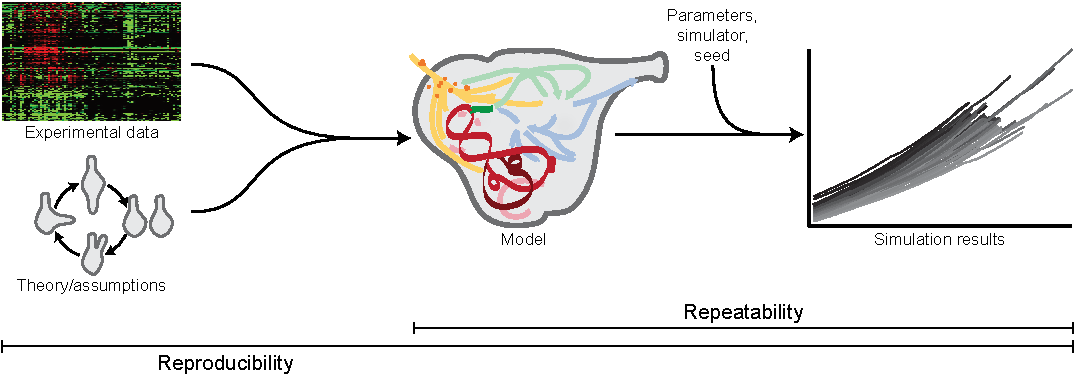
\includegraphics[width=\textwidth]{figure1/figure1}
% where an .eps filename suffix will be assumed under latex,
% and a .pdf suffix will be assumed for pdflatex; or what has been declared
% via \DeclareGraphicsExtensions.
\caption{Repeatability and reproducibility explained: Model reproducibility refers to derivation from scientific knowledge and the ability to generate results in a reliable, repeatable manner;
Repeatability refers only to the ability to recapitulate earlier simulation results}
\label{fig_repro_diagram}
\end{figure*}

\section{Repeatability and Reproducibility}

Fig.~\ref{fig_repro_diagram} shows the steps involved in reproducing a model. A subset of these steps involve replication only. To summarize these steps, the model's equations and parameter values must be duplicated from the original assumptions and experimental data. This requires machine-readable standards for concretely describing model components in terms of external database entries such as KEGG \cite{kanehisa2000kegg} compounds and MetaCyc \cite{caspi2008metacyc} reactions, machine-readable databases for representing the data sources that were used to parameterize a model, annotation standards for describing how those data sources were used to parameterize the model, and annotation standards for describing the assumptions that the model was based on \cite{boulton2012open}.

The result of the model construction steps described above will usually be a set of differential equations, reaction propensities, or rules which govern the timecourse behavior of the model. While in theory this formalism should be sufficient to recapitulate the model's behavior, we have found that reproducibility is further complicated by the details of the software implementation. In Matlab, for example, there are a number of differential equation solvers for both stiff and non-stiff systems. These solvers in turn have many configuration options relating to error tolerances and variable stepping. Therefore, we argue that software plays a critical role in reproducibility. Making the source code available helps to partly address this problem \cite{easterbrook2014open}, but we will show that more can be done to improve reproducibility in this area.

Stochastic models are problematic for reproducibility studies because they inherently give different output each time they are run. However, real implementations of stochastic processes often use pseudo-random number generators (PRNG) to achieve the illusion of stochasticity. The current standard for reproducing a stochastic model is based on comparing at least the first and second moments of the model's predictions. However, we argue that there are two advantages to reproducing the model's exact trajectory.

First, biology is replete with examples where rare events play key roles: e.g. cancer, speciation events, and mutations conferring antibiotic resistance. While these events may not occur often enough to contribute significantly to the expected dynamical behavior of a typical cell, they contribute significantly to the long-term behavior of the population. We believe that capturing these events when they occur will be instrumental to the usefullness of WC models as engines for discovery and prevention of such rare events.

Second, being able to reproduce a trace of model timecourse behavior is absolutely crucial to scaling up to large and complex models. Human error has been and will continue to be a major source of inaccuracy in modeling experiments \cite{ebrahim2015genome}. The ability to reproduce an exact model trace would be highly useful in the context of model reproduction endeavors such as the workshop by Waltemath and Schreiber because this ability allows modelers to identify the exact point at which predictions diverge. Assuming such errors occur at a constant rate, a larger model would be expected to contain many more errors than a smaller one, and eliminating such costly errors is a prerequisite to the adoption of WC modeling.

The idea of capturing the exact sequence of events leading to an error is not new. In the field of computer science, the SPIN model checker \cite{holzmann1997model} \cite{holzmann2004spin} has been used extensively to validate the operational logic of non-deterministic systems. SPIN detects invalid models by exhibiting a counterexample including the exact events leading to failure. We envisage a similar approach for biophysical modeling. Specifically, we envisage a simulator where not only can an exact simulation be replicated by supplying the same random seed, but also where a simulation may be restarted from a checkpoint containing a state snapshot at any point in the timecourse. Since serializing such checkpoints would be an expensive operation, the checkpoints would be user-specified. By combining these two features, we would be able to (1) replicate exactly a trace from a specific prior simulation, and (2) insert as many such checkpoints into the run as desired without affecting the outcome. We would then be able to capture rare events and apply permutations to test various hypotheses relating to the mechanism of the events, e.g. to test their robustness to knockouts and systematically screen for targets for intervention.

\subsection{Validation Tests as a Basis for Reproducibility}

Bergmann \cite{bergmann2008comparing} presented a strategy for comparing the outputs of various SBML ODE simulators, enabling developers of simulation tools to identify weaknesses of a particular implementation. The SBML Test Suite provides normative simulation output for specific SBML features\footnote{http://sbml.org/Software/SBML\_Test\_Suite}. Both of these tests cover ODE models only, which, owing to their determinism, can be reproduced across solvers. Hence, the criteria for passing these tests is whether the results converge to an \textit{a priori} known trajectory. Stochastic models, on the other hand, intrinsically do not converge to an exact trajectory. The current standard for testing stochastic models is a statistical test based on comparing the per-variable mean and standard deviation to expected values as a function of time \cite{evans2008sbml}.

In general, hybrid models contain both deterministic and stochastic components, so the statistical test could in principle be applicable. However, we argue that statistical tests are not sufficient to pronounce hybrid models (nor even complex stochastic ones) identical in practice. It has been shown that noise propagation in genetic networks can have a non-linear effect on the behavior of the network \cite{kim2013nonlinear}. A simple example is an $n$-stable switch (for example, a cell fate model) with noisy inputs. The system will ultimately end up in one of several stable states, dependent to a large extent on a random decision process. Consider a simple bi-stable switch. Over many trials, the sampled values of the variables of this system will exhibit bi-modality, with a mean in between the two modes and a very large variance encompassing the two modes, as shown in Fig.~\ref{fig_bistable_plot}. Rather than test whether a given trajectory fits within this large variance, a more useful test would be to confirm whether the trajectory follows one of the bi-modal patterns. However, complex models can contain many non-trivial features such as the aforementioned branching behavior and it is difficult to construct a generalized statistical test that encompasses all cases.

Insteady of relying on statistical tests, we propose that validation of hybrid models involve (1) independent validation of functional subunits based on whatever method is applicable, and (2) functional hypothesis-based testing for the hybrid model as a whole. For the first part, we assume subunits correspond models which can be simulated using a single solve (i.e. subunits are not themselves hybrid models). Hence, the tests outlined above for non-hybrid models may be applicable on a subunit basis, and will likely be sufficient in most cases. For testing the hybrid model as a whole, we resort to testing externally measurable outcomes for a given input or perturbation. For example, the cellular doubling time is externally measurable, and should respond in a predictable way to certain gene deletions under a given set of environmental conditions. These conditions are inputs to the model and can be reliably set up for the original model as well as any re-implementations. The outputs of these high-level tests should be the same across all implementations, and can serve as a measure of reproducibility. However, a failure in these high-level tests is difficult to trace back to its origin, underscoring the importance of the subunit tests. Hence, just as hybrid models follow a hierarchical construction, they must also follow a hierarchical validation scheme. This is the case for the \textit{M. genitalium} model (which contains many subunit tests under its \texttt{src\_test} directory), and we believe this approach will continue to be useful in future hybrid models.

\section{Constructing a Platform for Complex, Hybrid Modeling}

The \textit{M. genitalium} re-encoding effort provides a useful test case for a platform designed to support large, complex, hybrid models, such as WC models. Using the outcome of the workshop as an example, we can expect the following areas to be key features in the next generation of modeling software:

\begin{itemize}
\item A hybrid timecourse solver incorporating multiple, heterogeneous codebases
\item Better standards for model integration, including how to parallelize the model for execution performance
\item Transparent encoding of model data and initialization
\end{itemize}

These focus areas require advances in simulation software, standards, and services to connect models and data. The first requirement necessitates having a way for a diverse set of solvers to communicate. There are many ways to achieve this, including shared memory buffers, memory-mapped files, or message passing. Message passing offers the additional advantage that the different solvers can reside on different machines connected by a network. Furthermore, if the structure of the data contained in the message is defined and documented, it is possible to use the message passing scheme from many different programming languages and software environments. The SBML Arrays package \cite{watanabe2016efficient} helps aid in the parallelization of certain types of models, while the Hierarchical Model Composition package \cite{smith2015sbml} offers a way to integrate models. However, there is overlap between these two packages, and their respective feature sets could be reconciled into a single scheme for encoding and simulating hierarchical models. This scheme must also address how to deal with updates to shared variables, which can be a source of conflicts and race conditions. Finally, better databases and services are needed to transparently, unambiguously tie the parameterization and initialization of the model to the data used to generate it. Linked data has proven to be extremely useful both in the annotation of XML-encoded standards \cite{novere2005minimum} and pure RDF standards \cite{galdzicki2014synthetic}.

Before a platform for hybrid modeling can be realized, the modeling community will first need to agree on a few preliminary features such a platform should have. For a hybrid solver to be useful, it should be implemented as a highly reusable software system. In so far as possible, it should be language-agnostic in order to reach the broadest possible audience. As an example, consider Geppetto, the multi-solver interface for the OpenWorm project \footnote{http://www.openworm.org/}. Geppetto uses the OSGi framework to interface with various solvers in a modular way. However, this system has a serious drawback: It is not language agnostic, and requires an OSGi interface written in Java for each component. This in turn imposes a burden on developers of non-Java solvers. While we are not aware of any single system that can address all of OSGi's use cases in a language agnostic way, we do acknowledge that there are libraries (such as ZeroMQ) that enable cross-process and cross-platform communication, and we believe that using communication as the starting point and building a service architecture on top of it is more language agnostic than starting with a specific service scheme (OSGi) and trying to build a system for cross-language communication.

It has been our experience that non-replicable simulations are notoriously difficult to debug. Therefore, we propose that in order to build a scalable platform, replicable simulations should be incorporated as a core feature. Since replicable simulations are difficult to achieve for hybrid models with the aforementioned synchronization issues for shared variables, we devote an entire section to this problem and how it is handled in computer science. We then suggest how these computer science techniques may be applied to timecourse simulation software.

\begin{figure*}[!t]
  \centering
  \begin{subfigure}[t]{0.5\textwidth}
    \centering
    % This file was created by matplotlib2tikz v0.5.4.
% The lastest updates can be retrieved from
% 
% https://github.com/nschloe/matplotlib2tikz
% 
% where you can also submit bug reports and leavecomments.
% 
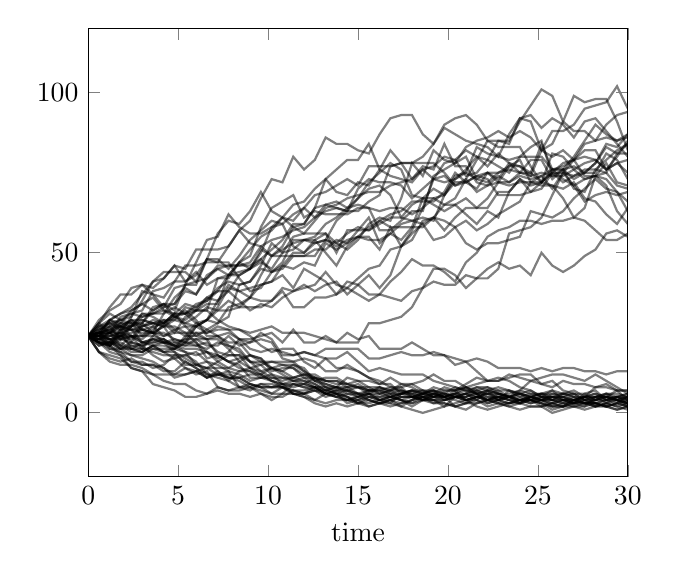
\begin{tikzpicture}

\begin{axis}[
xlabel={time},
xmin=0, xmax=30,
ymin=-20, ymax=120,
axis on top
]
\addplot [thick, black, opacity=0.5]
table {%
0 23.88
0.6 23.88
1.2 20.88
1.8 18.88
2.4 17.88
3 16.88
3.6 15.88
4.2 13.88
4.8 10.88
5.4 11.88
6 12.88
6.6 10.88
7.2 11.88
7.8 10.88
8.4 9.88
9 7.88
9.6 8.88
10.2 7.88
10.8 7.88
11.4 5.88
12 4.88
12.6 3.88
13.2 5.88
13.8 4.88
14.4 3.88
15 4.88
15.6 5.88
16.2 3.88
16.8 4.88
17.4 3.88
18 4.88
18.6 3.88
19.2 4.88
19.8 6.88
20.4 6.88
21 7.88
21.6 5.88
22.2 3.88
22.8 4.88
23.4 5.88
24 6.88
24.6 9.88
25.2 8.88
25.8 9.88
26.4 6.88
27 5.88
27.6 5.88
28.2 3.88
28.8 5.88
29.4 4.88
30 3.88
};
\addplot [thick, black, opacity=0.5]
table {%
0 23.88
0.6 23.88
1.2 28.88
1.8 30.88
2.4 31.88
3 33.88
3.6 31.88
4.2 33.88
4.8 33.88
5.4 39.88
6 46.88
6.6 53.88
7.2 54.88
7.8 61.88
8.4 57.88
9 55.88
9.6 55.88
10.2 57.88
10.8 60.88
11.4 57.88
12 58.88
12.6 63.88
13.2 64.88
13.8 65.88
14.4 63.88
15 64.88
15.6 63.88
16.2 56.88
16.8 56.88
17.4 59.88
18 62.88
18.6 62.88
19.2 73.88
19.8 75.88
20.4 77.88
21 82.88
21.6 84.88
22.2 85.88
22.8 87.88
23.4 85.88
24 87.88
24.6 85.88
25.2 81.88
25.8 87.88
26.4 87.88
27 89.88
27.6 94.88
28.2 95.88
28.8 96.88
29.4 101.88
30 94.88
};
\addplot [thick, black, opacity=0.5]
table {%
0 23.88
0.6 24.88
1.2 24.88
1.8 25.88
2.4 26.88
3 27.88
3.6 24.88
4.2 24.88
4.8 22.88
5.4 21.88
6 20.88
6.6 19.88
7.2 21.88
7.8 20.88
8.4 19.88
9 15.88
9.6 15.88
10.2 13.88
10.8 12.88
11.4 10.88
12 11.88
12.6 9.88
13.2 10.88
13.8 10.88
14.4 8.88
15 7.88
15.6 6.88
16.2 6.88
16.8 5.88
17.4 3.88
18 1.88
18.6 3.88
19.2 3.88
19.8 2.88
20.4 1.88
21 0.879999999999999
21.6 2.88
22.2 3.88
22.8 5.88
23.4 4.88
24 3.88
24.6 4.88
25.2 3.88
25.8 2.88
26.4 3.88
27 2.88
27.6 2.88
28.2 1.88
28.8 2.88
29.4 1.88
30 0.879999999999999
};
\addplot [thick, black, opacity=0.5]
table {%
0 23.88
0.6 23.88
1.2 24.88
1.8 29.88
2.4 30.88
3 31.88
3.6 37.88
4.2 38.88
4.8 40.88
5.4 45.88
6 45.88
6.6 46.88
7.2 46.88
7.8 46.88
8.4 41.88
9 37.88
9.6 38.88
10.2 43.88
10.8 46.88
11.4 53.88
12 53.88
12.6 54.88
13.2 58.88
13.8 60.88
14.4 63.88
15 66.88
15.6 71.88
16.2 74.88
16.8 77.88
17.4 75.88
18 67.88
18.6 66.88
19.2 64.88
19.8 62.88
20.4 64.88
21 66.88
21.6 63.88
22.2 66.88
22.8 71.88
23.4 76.88
24 76.88
24.6 74.88
25.2 71.88
25.8 80.88
26.4 79.88
27 75.88
27.6 72.88
28.2 73.88
28.8 70.88
29.4 62.88
30 58.88
};
\addplot [thick, black, opacity=0.5]
table {%
0 23.88
0.6 23.88
1.2 26.88
1.8 26.88
2.4 23.88
3 19.88
3.6 18.88
4.2 17.88
4.8 17.88
5.4 15.88
6 13.88
6.6 11.88
7.2 11.88
7.8 10.88
8.4 10.88
9 11.88
9.6 11.88
10.2 13.88
10.8 11.88
11.4 9.88
12 9.88
12.6 8.88
13.2 6.88
13.8 5.88
14.4 4.88
15 2.88
15.6 3.88
16.2 2.88
16.8 3.88
17.4 4.88
18 4.88
18.6 3.88
19.2 4.88
19.8 5.88
20.4 7.88
21 6.88
21.6 5.88
22.2 3.88
22.8 2.88
23.4 1.88
24 2.88
24.6 4.88
25.2 3.88
25.8 4.88
26.4 5.88
27 6.88
27.6 4.88
28.2 4.88
28.8 4.88
29.4 3.88
30 2.88
};
\addplot [thick, black, opacity=0.5]
table {%
0 23.88
0.6 25.88
1.2 27.88
1.8 26.88
2.4 28.88
3 26.88
3.6 27.88
4.2 26.88
4.8 29.88
5.4 28.88
6 31.88
6.6 31.88
7.2 41.88
7.8 41.88
8.4 46.88
9 50.88
9.6 54.88
10.2 56.88
10.8 60.88
11.4 59.88
12 63.88
12.6 60.88
13.2 62.88
13.8 63.88
14.4 62.88
15 69.88
15.6 72.88
16.2 71.88
16.8 71.88
17.4 70.88
18 66.88
18.6 69.88
19.2 72.88
19.8 77.88
20.4 78.88
21 73.88
21.6 74.88
22.2 78.88
22.8 76.88
23.4 74.88
24 79.88
24.6 82.88
25.2 84.88
25.8 73.88
26.4 73.88
27 75.88
27.6 77.88
28.2 78.88
28.8 75.88
29.4 77.88
30 74.88
};
\addplot [thick, black, opacity=0.5]
table {%
0 23.88
0.6 24.88
1.2 24.88
1.8 26.88
2.4 25.88
3 21.88
3.6 22.88
4.2 21.88
4.8 18.88
5.4 16.88
6 14.88
6.6 15.88
7.2 14.88
7.8 12.88
8.4 7.88
9 8.88
9.6 7.88
10.2 7.88
10.8 7.88
11.4 5.88
12 5.88
12.6 6.88
13.2 6.88
13.8 5.88
14.4 2.88
15 3.88
15.6 1.88
16.2 2.88
16.8 3.88
17.4 2.88
18 3.88
18.6 4.88
19.2 2.88
19.8 3.88
20.4 4.88
21 3.88
21.6 3.88
22.2 1.88
22.8 2.88
23.4 1.88
24 0.879999999999999
24.6 1.88
25.2 1.88
25.8 2.88
26.4 3.88
27 3.88
27.6 2.88
28.2 3.88
28.8 4.88
29.4 3.88
30 2.88
};
\addplot [thick, black, opacity=0.5]
table {%
0 23.88
0.6 21.88
1.2 21.88
1.8 19.88
2.4 20.88
3 19.88
3.6 19.88
4.2 18.88
4.8 19.88
5.4 18.88
6 17.88
6.6 18.88
7.2 15.88
7.8 13.88
8.4 12.88
9 13.88
9.6 12.88
10.2 10.88
10.8 9.88
11.4 10.88
12 9.88
12.6 7.88
13.2 5.88
13.8 4.88
14.4 5.88
15 5.88
15.6 5.88
16.2 4.88
16.8 4.88
17.4 3.88
18 2.88
18.6 3.88
19.2 3.88
19.8 1.88
20.4 4.88
21 4.88
21.6 6.88
22.2 4.88
22.8 4.88
23.4 4.88
24 4.88
24.6 3.88
25.2 1.88
25.8 -0.120000000000001
26.4 0.879999999999999
27 1.88
27.6 2.88
28.2 2.88
28.8 1.88
29.4 0.879999999999999
30 1.88
};
\addplot [thick, black, opacity=0.5]
table {%
0 23.88
0.6 27.88
1.2 32.88
1.8 36.88
2.4 36.88
3 39.88
3.6 38.88
4.2 41.88
4.8 45.88
5.4 40.88
6 42.88
6.6 47.88
7.2 55.88
7.8 59.88
8.4 58.88
9 62.88
9.6 68.88
10.2 62.88
10.8 60.88
11.4 64.88
12 65.88
12.6 69.88
13.2 72.88
13.8 68.88
14.4 67.88
15 71.88
15.6 70.88
16.2 75.88
16.8 73.88
17.4 72.88
18 71.88
18.6 75.88
19.2 72.88
19.8 71.88
20.4 72.88
21 74.88
21.6 72.88
22.2 71.88
22.8 74.88
23.4 76.88
24 78.88
24.6 71.88
25.2 73.88
25.8 75.88
26.4 76.88
27 78.88
27.6 73.88
28.2 73.88
28.8 72.88
29.4 68.88
30 62.88
};
\addplot [thick, black, opacity=0.5]
table {%
0 23.88
0.6 23.88
1.2 23.88
1.8 24.88
2.4 29.88
3 34.88
3.6 40.88
4.2 43.88
4.8 43.88
5.4 43.88
6 40.88
6.6 47.88
7.2 47.88
7.8 44.88
8.4 48.88
9 53.88
9.6 56.88
10.2 59.88
10.8 58.88
11.4 51.88
12 49.88
12.6 52.88
13.2 53.88
13.8 51.88
14.4 53.88
15 54.88
15.6 53.88
16.2 53.88
16.8 55.88
17.4 53.88
18 57.88
18.6 66.88
19.2 69.88
19.8 67.88
20.4 72.88
21 75.88
21.6 79.88
22.2 76.88
22.8 80.88
23.4 77.88
24 74.88
24.6 73.88
25.2 74.88
25.8 73.88
26.4 75.88
27 69.88
27.6 68.88
28.2 75.88
28.8 78.88
29.4 81.88
30 83.88
};
\addplot [thick, black, opacity=0.5]
table {%
0 23.88
0.6 21.88
1.2 20.88
1.8 22.88
2.4 23.88
3 22.88
3.6 25.88
4.2 28.88
4.8 28.88
5.4 32.88
6 31.88
6.6 35.88
7.2 34.88
7.8 37.88
8.4 42.88
9 44.88
9.6 49.88
10.2 57.88
10.8 58.88
11.4 61.88
12 63.88
12.6 67.88
13.2 68.88
13.8 70.88
14.4 72.88
15 70.88
15.6 76.88
16.2 76.88
16.8 76.88
17.4 77.88
18 72.88
18.6 75.88
19.2 76.88
19.8 79.88
20.4 78.88
21 81.88
21.6 79.88
22.2 78.88
22.8 84.88
23.4 84.88
24 90.88
24.6 95.88
25.2 100.88
25.8 98.88
26.4 90.88
27 98.88
27.6 96.88
28.2 97.88
28.8 97.88
29.4 90.88
30 81.88
};
\addplot [thick, black, opacity=0.5]
table {%
0 23.88
0.6 24.88
1.2 25.88
1.8 26.88
2.4 26.88
3 30.88
3.6 30.88
4.2 32.88
4.8 33.88
5.4 37.88
6 36.88
6.6 41.88
7.2 44.88
7.8 45.88
8.4 45.88
9 45.88
9.6 47.88
10.2 43.88
10.8 44.88
11.4 48.88
12 48.88
12.6 48.88
13.2 53.88
13.8 52.88
14.4 55.88
15 57.88
15.6 56.88
16.2 59.88
16.8 57.88
17.4 57.88
18 57.88
18.6 57.88
19.2 60.88
19.8 59.88
20.4 57.88
21 52.88
21.6 50.88
22.2 52.88
22.8 52.88
23.4 53.88
24 54.88
24.6 62.88
25.2 61.88
25.8 60.88
26.4 62.88
27 66.88
27.6 69.88
28.2 72.88
28.8 69.88
29.4 68.88
30 65.88
};
\addplot [thick, black, opacity=0.5]
table {%
0 23.88
0.6 25.88
1.2 27.88
1.8 28.88
2.4 30.88
3 29.88
3.6 30.88
4.2 31.88
4.8 29.88
5.4 30.88
6 32.88
6.6 35.88
7.2 37.88
7.8 42.88
8.4 46.88
9 48.88
9.6 57.88
10.2 63.88
10.8 65.88
11.4 67.88
12 60.88
12.6 62.88
13.2 61.88
13.8 61.88
14.4 61.88
15 63.88
15.6 63.88
16.2 62.88
16.8 63.88
17.4 63.88
18 61.88
18.6 63.88
19.2 66.88
19.8 64.88
20.4 64.88
21 61.88
21.6 58.88
22.2 62.88
22.8 60.88
23.4 68.88
24 72.88
24.6 68.88
25.2 69.88
25.8 74.88
26.4 77.88
27 78.88
27.6 81.88
28.2 81.88
28.8 75.88
29.4 79.88
30 84.88
};
\addplot [thick, black, opacity=0.5]
table {%
0 23.88
0.6 24.88
1.2 26.88
1.8 22.88
2.4 26.88
3 28.88
3.6 27.88
4.2 28.88
4.8 25.88
5.4 26.88
6 23.88
6.6 22.88
7.2 23.88
7.8 24.88
8.4 22.88
9 21.88
9.6 22.88
10.2 21.88
10.8 16.88
11.4 15.88
12 16.88
12.6 15.88
13.2 12.88
13.8 12.88
14.4 14.88
15 12.88
15.6 10.88
16.2 9.88
16.8 7.88
17.4 7.88
18 4.88
18.6 5.88
19.2 6.88
19.8 4.88
20.4 5.88
21 5.88
21.6 7.88
22.2 6.88
22.8 3.88
23.4 2.88
24 2.88
24.6 1.88
25.2 1.88
25.8 2.88
26.4 1.88
27 3.88
27.6 4.88
28.2 4.88
28.8 2.88
29.4 3.88
30 2.88
};
\addplot [thick, black, opacity=0.5]
table {%
0 23.88
0.6 20.88
1.2 21.88
1.8 20.88
2.4 18.88
3 18.88
3.6 20.88
4.2 20.88
4.8 19.88
5.4 23.88
6 23.88
6.6 25.88
7.2 27.88
7.8 32.88
8.4 33.88
9 35.88
9.6 42.88
10.2 48.88
10.8 51.88
11.4 57.88
12 55.88
12.6 59.88
13.2 63.88
13.8 64.88
14.4 66.88
15 67.88
15.6 68.88
16.2 68.88
16.8 70.88
17.4 71.88
18 72.88
18.6 76.88
19.2 75.88
19.8 83.88
20.4 76.88
21 76.88
21.6 71.88
22.2 70.88
22.8 71.88
23.4 70.88
24 71.88
24.6 71.88
25.2 71.88
25.8 70.88
26.4 66.88
27 60.88
27.6 63.88
28.2 73.88
28.8 77.88
29.4 71.88
30 70.88
};
\addplot [thick, black, opacity=0.5]
table {%
0 23.88
0.6 18.88
1.2 15.88
1.8 14.88
2.4 14.88
3 13.88
3.6 11.88
4.2 11.88
4.8 11.88
5.4 13.88
6 11.88
6.6 12.88
7.2 7.88
7.8 6.88
8.4 6.88
9 7.88
9.6 5.88
10.2 3.88
10.8 5.88
11.4 8.88
12 7.88
12.6 6.88
13.2 5.88
13.8 6.88
14.4 4.88
15 2.88
15.6 4.88
16.2 3.88
16.8 3.88
17.4 1.88
18 0.879999999999999
18.6 -0.120000000000001
19.2 0.879999999999999
19.8 1.88
20.4 2.88
21 3.88
21.6 4.88
22.2 5.88
22.8 6.88
23.4 6.88
24 5.88
24.6 6.88
25.2 4.88
25.8 3.88
26.4 2.88
27 2.88
27.6 5.88
28.2 6.88
28.8 3.88
29.4 4.88
30 5.88
};
\addplot [thick, black, opacity=0.5]
table {%
0 23.88
0.6 24.88
1.2 23.88
1.8 24.88
2.4 23.88
3 23.88
3.6 26.88
4.2 27.88
4.8 30.88
5.4 33.88
6 32.88
6.6 34.88
7.2 38.88
7.8 40.88
8.4 39.88
9 40.88
9.6 44.88
10.2 43.88
10.8 45.88
11.4 49.88
12 49.88
12.6 53.88
13.2 55.88
13.8 49.88
14.4 56.88
15 56.88
15.6 56.88
16.2 58.88
16.8 60.88
17.4 60.88
18 59.88
18.6 58.88
19.2 60.88
19.8 64.88
20.4 66.88
21 72.88
21.6 78.88
22.2 84.88
22.8 82.88
23.4 82.88
24 82.88
24.6 76.88
25.2 71.88
25.8 75.88
26.4 72.88
27 70.88
27.6 65.88
28.2 67.88
28.8 68.88
29.4 67.88
30 68.88
};
\addplot [thick, black, opacity=0.5]
table {%
0 23.88
0.6 24.88
1.2 22.88
1.8 23.88
2.4 24.88
3 25.88
3.6 24.88
4.2 21.88
4.8 22.88
5.4 21.88
6 21.88
6.6 16.88
7.2 17.88
7.8 15.88
8.4 16.88
9 17.88
9.6 16.88
10.2 13.88
10.8 14.88
11.4 13.88
12 11.88
12.6 10.88
13.2 7.88
13.8 7.88
14.4 6.88
15 4.88
15.6 5.88
16.2 7.88
16.8 5.88
17.4 6.88
18 5.88
18.6 4.88
19.2 3.88
19.8 4.88
20.4 6.88
21 7.88
21.6 5.88
22.2 6.88
22.8 5.88
23.4 4.88
24 3.88
24.6 4.88
25.2 3.88
25.8 3.88
26.4 3.88
27 2.88
27.6 3.88
28.2 2.88
28.8 3.88
29.4 4.88
30 3.88
};
\addplot [thick, black, opacity=0.5]
table {%
0 23.88
0.6 21.88
1.2 19.88
1.8 19.88
2.4 21.88
3 26.88
3.6 27.88
4.2 26.88
4.8 21.88
5.4 22.88
6 22.88
6.6 20.88
7.2 20.88
7.8 23.88
8.4 20.88
9 21.88
9.6 24.88
10.2 22.88
10.8 17.88
11.4 17.88
12 18.88
12.6 17.88
13.2 16.88
13.8 16.88
14.4 18.88
15 15.88
15.6 12.88
16.2 13.88
16.8 12.88
17.4 11.88
18 11.88
18.6 11.88
19.2 9.88
19.8 8.88
20.4 7.88
21 6.88
21.6 7.88
22.2 7.88
22.8 5.88
23.4 4.88
24 5.88
24.6 3.88
25.2 4.88
25.8 3.88
26.4 4.88
27 2.88
27.6 3.88
28.2 1.88
28.8 2.88
29.4 4.88
30 2.88
};
\addplot [thick, black, opacity=0.5]
table {%
0 23.88
0.6 23.88
1.2 22.88
1.8 23.88
2.4 22.88
3 27.88
3.6 31.88
4.2 33.88
4.8 31.88
5.4 39.88
6 39.88
6.6 47.88
7.2 46.88
7.8 51.88
8.4 56.88
9 59.88
9.6 66.88
10.2 72.88
10.8 71.88
11.4 79.88
12 75.88
12.6 78.88
13.2 85.88
13.8 83.88
14.4 83.88
15 81.88
15.6 80.88
16.2 86.88
16.8 91.88
17.4 92.88
18 92.88
18.6 86.88
19.2 83.88
19.8 89.88
20.4 91.88
21 92.88
21.6 89.88
22.2 84.88
22.8 84.88
23.4 83.88
24 91.88
24.6 90.88
25.2 81.88
25.8 83.88
26.4 90.88
27 87.88
27.6 87.88
28.2 84.88
28.8 85.88
29.4 84.88
30 85.88
};
\addplot [thick, black, opacity=0.5]
table {%
0 23.88
0.6 24.88
1.2 28.88
1.8 30.88
2.4 32.88
3 36.88
3.6 40.88
4.2 41.88
4.8 45.88
5.4 44.88
6 50.88
6.6 50.88
7.2 50.88
7.8 51.88
8.4 56.88
9 52.88
9.6 51.88
10.2 48.88
10.8 50.88
11.4 52.88
12 53.88
12.6 52.88
13.2 53.88
13.8 59.88
14.4 62.88
15 62.88
15.6 65.88
16.2 67.88
16.8 76.88
17.4 77.88
18 77.88
18.6 79.88
19.2 83.88
19.8 88.88
20.4 86.88
21 84.88
21.6 83.88
22.2 82.88
22.8 79.88
23.4 86.88
24 91.88
24.6 92.88
25.2 88.88
25.8 91.88
26.4 89.88
27 85.88
27.6 90.88
28.2 91.88
28.8 87.88
29.4 83.88
30 79.88
};
\addplot [thick, black, opacity=0.5]
table {%
0 23.88
0.6 24.88
1.2 20.88
1.8 24.88
2.4 25.88
3 24.88
3.6 24.88
4.2 26.88
4.8 28.88
5.4 27.88
6 26.88
6.6 24.88
7.2 26.88
7.8 25.88
8.4 25.88
9 23.88
9.6 20.88
10.2 18.88
10.8 19.88
11.4 19.88
12 15.88
12.6 13.88
13.2 16.88
13.8 13.88
14.4 13.88
15 12.88
15.6 10.88
16.2 8.88
16.8 8.88
17.4 5.88
18 6.88
18.6 5.88
19.2 6.88
19.8 5.88
20.4 4.88
21 5.88
21.6 6.88
22.2 7.88
22.8 6.88
23.4 4.88
24 3.88
24.6 3.88
25.2 4.88
25.8 4.88
26.4 4.88
27 3.88
27.6 2.88
28.2 1.88
28.8 1.88
29.4 2.88
30 1.88
};
\addplot [thick, black, opacity=0.5]
table {%
0 23.88
0.6 21.88
1.2 20.88
1.8 23.88
2.4 27.88
3 23.88
3.6 24.88
4.2 26.88
4.8 26.88
5.4 24.88
6 24.88
6.6 22.88
7.2 17.88
7.8 15.88
8.4 13.88
9 12.88
9.6 10.88
10.2 9.88
10.8 7.88
11.4 6.88
12 6.88
12.6 7.88
13.2 6.88
13.8 7.88
14.4 5.88
15 4.88
15.6 6.88
16.2 6.88
16.8 7.88
17.4 6.88
18 5.88
18.6 3.88
19.2 5.88
19.8 7.88
20.4 6.88
21 3.88
21.6 4.88
22.2 4.88
22.8 3.88
23.4 4.88
24 3.88
24.6 4.88
25.2 3.88
25.8 1.88
26.4 1.88
27 2.88
27.6 2.88
28.2 3.88
28.8 3.88
29.4 2.88
30 3.88
};
\addplot [thick, black, opacity=0.5]
table {%
0 23.88
0.6 22.88
1.2 22.88
1.8 20.88
2.4 23.88
3 21.88
3.6 22.88
4.2 22.88
4.8 19.88
5.4 21.88
6 24.88
6.6 24.88
7.2 25.88
7.8 25.88
8.4 22.88
9 19.88
9.6 18.88
10.2 19.88
10.8 18.88
11.4 17.88
12 18.88
12.6 17.88
13.2 19.88
13.8 19.88
14.4 19.88
15 19.88
15.6 16.88
16.2 16.88
16.8 17.88
17.4 18.88
18 17.88
18.6 17.88
19.2 18.88
19.8 17.88
20.4 16.88
21 15.88
21.6 12.88
22.2 9.88
22.8 9.88
23.4 11.88
24 10.88
24.6 9.88
25.2 10.88
25.8 11.88
26.4 11.88
27 10.88
27.6 9.88
28.2 11.88
28.8 9.88
29.4 7.88
30 5.88
};
\addplot [thick, black, opacity=0.5]
table {%
0 23.88
0.6 21.88
1.2 21.88
1.8 25.88
2.4 25.88
3 26.88
3.6 28.88
4.2 27.88
4.8 24.88
5.4 29.88
6 31.88
6.6 33.88
7.2 33.88
7.8 42.88
8.4 43.88
9 44.88
9.6 47.88
10.2 50.88
10.8 53.88
11.4 58.88
12 58.88
12.6 63.88
13.2 72.88
13.8 75.88
14.4 78.88
15 78.88
15.6 83.88
16.2 75.88
16.8 81.88
17.4 77.88
18 77.88
18.6 77.88
19.2 77.88
19.8 74.88
20.4 70.88
21 72.88
21.6 68.88
22.2 70.88
22.8 73.88
23.4 71.88
24 73.88
24.6 72.88
25.2 73.88
25.8 69.88
26.4 74.88
27 78.88
27.6 79.88
28.2 78.88
28.8 75.88
29.4 77.88
30 78.88
};
\addplot [thick, black, opacity=0.5]
table {%
0 23.88
0.6 27.88
1.2 24.88
1.8 27.88
2.4 31.88
3 33.88
3.6 35.88
4.2 31.88
4.8 30.88
5.4 30.88
6 27.88
6.6 28.88
7.2 27.88
7.8 29.88
8.4 39.88
9 40.88
9.6 45.88
10.2 52.88
10.8 49.88
11.4 50.88
12 53.88
12.6 53.88
13.2 49.88
13.8 45.88
14.4 51.88
15 54.88
15.6 54.88
16.2 50.88
16.8 57.88
17.4 51.88
18 55.88
18.6 58.88
19.2 53.88
19.8 54.88
20.4 57.88
21 59.88
21.6 56.88
22.2 58.88
22.8 61.88
23.4 63.88
24 65.88
24.6 71.88
25.2 70.88
25.8 70.88
26.4 69.88
27 71.88
27.6 66.88
28.2 65.88
28.8 61.88
29.4 58.88
30 63.88
};
\addplot [thick, black, opacity=0.5]
table {%
0 23.88
0.6 18.88
1.2 16.88
1.8 15.88
2.4 16.88
3 14.88
3.6 14.88
4.2 12.88
4.8 12.88
5.4 15.88
6 13.88
6.6 10.88
7.2 12.88
7.8 9.88
8.4 12.88
9 12.88
9.6 11.88
10.2 9.88
10.8 8.88
11.4 9.88
12 10.88
12.6 10.88
13.2 8.88
13.8 7.88
14.4 10.88
15 9.88
15.6 7.88
16.2 7.88
16.8 6.88
17.4 4.88
18 4.88
18.6 5.88
19.2 4.88
19.8 5.88
20.4 4.88
21 4.88
21.6 5.88
22.2 6.88
22.8 5.88
23.4 4.88
24 2.88
24.6 4.88
25.2 3.88
25.8 2.88
26.4 1.88
27 2.88
27.6 4.88
28.2 5.88
28.8 3.88
29.4 4.88
30 5.88
};
\addplot [thick, black, opacity=0.5]
table {%
0 23.88
0.6 22.88
1.2 24.88
1.8 24.88
2.4 19.88
3 19.88
3.6 23.88
4.2 27.88
4.8 29.88
5.4 27.88
6 29.88
6.6 32.88
7.2 31.88
7.8 31.88
8.4 32.88
9 32.88
9.6 32.88
10.2 34.88
10.8 38.88
11.4 37.88
12 39.88
12.6 37.88
13.2 39.88
13.8 40.88
14.4 36.88
15 39.88
15.6 42.88
16.2 38.88
16.8 42.88
17.4 51.88
18 56.88
18.6 63.88
19.2 72.88
19.8 73.88
20.4 70.88
21 71.88
21.6 73.88
22.2 72.88
22.8 67.88
23.4 67.88
24 67.88
24.6 68.88
25.2 71.88
25.8 74.88
26.4 74.88
27 70.88
27.6 72.88
28.2 73.88
28.8 74.88
29.4 70.88
30 69.88
};
\addplot [thick, black, opacity=0.5]
table {%
0 23.88
0.6 26.88
1.2 27.88
1.8 25.88
2.4 28.88
3 28.88
3.6 27.88
4.2 27.88
4.8 30.88
5.4 30.88
6 33.88
6.6 34.88
7.2 37.88
7.8 37.88
8.4 34.88
9 31.88
9.6 33.88
10.2 32.88
10.8 35.88
11.4 37.88
12 38.88
12.6 39.88
13.2 43.88
13.8 39.88
14.4 38.88
15 36.88
15.6 34.88
16.2 36.88
16.8 40.88
17.4 43.88
18 47.88
18.6 45.88
19.2 45.88
19.8 43.88
20.4 40.88
21 46.88
21.6 49.88
22.2 54.88
22.8 56.88
23.4 57.88
24 59.88
24.6 59.88
25.2 58.88
25.8 59.88
26.4 59.88
27 60.88
27.6 59.88
28.2 56.88
28.8 53.88
29.4 53.88
30 55.88
};
\addplot [thick, black, opacity=0.5]
table {%
0 23.88
0.6 21.88
1.2 20.88
1.8 17.88
2.4 15.88
3 15.88
3.6 13.88
4.2 14.88
4.8 17.88
5.4 17.88
6 15.88
6.6 11.88
7.2 10.88
7.8 9.88
8.4 7.88
9 6.88
9.6 8.88
10.2 8.88
10.8 7.88
11.4 8.88
12 7.88
12.6 7.88
13.2 5.88
13.8 4.88
14.4 3.88
15 4.88
15.6 3.88
16.2 2.88
16.8 2.88
17.4 5.88
18 6.88
18.6 5.88
19.2 4.88
19.8 3.88
20.4 4.88
21 3.88
21.6 1.88
22.2 0.879999999999999
22.8 1.88
23.4 2.88
24 3.88
24.6 2.88
25.2 3.88
25.8 4.88
26.4 3.88
27 3.88
27.6 4.88
28.2 7.88
28.8 7.88
29.4 6.88
30 6.88
};
\addplot [thick, black, opacity=0.5]
table {%
0 23.88
0.6 24.88
1.2 21.88
1.8 21.88
2.4 19.88
3 21.88
3.6 20.88
4.2 21.88
4.8 20.88
5.4 18.88
6 14.88
6.6 13.88
7.2 13.88
7.8 13.88
8.4 15.88
9 13.88
9.6 14.88
10.2 11.88
10.8 10.88
11.4 9.88
12 8.88
12.6 7.88
13.2 5.88
13.8 5.88
14.4 3.88
15 2.88
15.6 1.88
16.2 2.88
16.8 1.88
17.4 2.88
18 3.88
18.6 5.88
19.2 7.88
19.8 6.88
20.4 6.88
21 8.88
21.6 10.88
22.2 9.88
22.8 10.88
23.4 9.88
24 7.88
24.6 6.88
25.2 4.88
25.8 6.88
26.4 3.88
27 4.88
27.6 3.88
28.2 4.88
28.8 4.88
29.4 3.88
30 2.88
};
\addplot [thick, black, opacity=0.5]
table {%
0 23.88
0.6 24.88
1.2 28.88
1.8 27.88
2.4 26.88
3 30.88
3.6 29.88
4.2 27.88
4.8 30.88
5.4 26.88
6 26.88
6.6 28.88
7.2 31.88
7.8 34.88
8.4 32.88
9 35.88
9.6 34.88
10.2 34.88
10.8 37.88
11.4 32.88
12 32.88
12.6 35.88
13.2 35.88
13.8 36.88
14.4 40.88
15 39.88
15.6 36.88
16.2 36.88
16.8 35.88
17.4 34.88
18 37.88
18.6 38.88
19.2 44.88
19.8 44.88
20.4 42.88
21 38.88
21.6 41.88
22.2 44.88
22.8 46.88
23.4 44.88
24 45.88
24.6 42.88
25.2 49.88
25.8 45.88
26.4 43.88
27 45.88
27.6 48.88
28.2 50.88
28.8 55.88
29.4 56.88
30 54.88
};
\addplot [thick, black, opacity=0.5]
table {%
0 23.88
0.6 22.88
1.2 21.88
1.8 23.88
2.4 26.88
3 29.88
3.6 30.88
4.2 30.88
4.8 32.88
5.4 30.88
6 31.88
6.6 31.88
7.2 28.88
7.8 26.88
8.4 25.88
9 24.88
9.6 25.88
10.2 26.88
10.8 24.88
11.4 24.88
12 24.88
12.6 23.88
13.2 22.88
13.8 21.88
14.4 24.88
15 22.88
15.6 23.88
16.2 19.88
16.8 19.88
17.4 19.88
18 21.88
18.6 19.88
19.2 17.88
19.8 17.88
20.4 14.88
21 15.88
21.6 16.88
22.2 15.88
22.8 13.88
23.4 13.88
24 13.88
24.6 12.88
25.2 13.88
25.8 12.88
26.4 13.88
27 13.88
27.6 12.88
28.2 12.88
28.8 11.88
29.4 12.88
30 12.88
};
\addplot [thick, black, opacity=0.5]
table {%
0 23.88
0.6 24.88
1.2 25.88
1.8 23.88
2.4 23.88
3 21.88
3.6 21.88
4.2 21.88
4.8 20.88
5.4 20.88
6 22.88
6.6 22.88
7.2 22.88
7.8 19.88
8.4 15.88
9 17.88
9.6 15.88
10.2 15.88
10.8 15.88
11.4 15.88
12 12.88
12.6 10.88
13.2 9.88
13.8 9.88
14.4 8.88
15 9.88
15.6 9.88
16.2 8.88
16.8 10.88
17.4 8.88
18 8.88
18.6 9.88
19.2 11.88
19.8 9.88
20.4 9.88
21 7.88
21.6 8.88
22.2 9.88
22.8 9.88
23.4 10.88
24 11.88
24.6 11.88
25.2 8.88
25.8 7.88
26.4 9.88
27 8.88
27.6 8.88
28.2 7.88
28.8 8.88
29.4 6.88
30 3.88
};
\addplot [thick, black, opacity=0.5]
table {%
0 23.88
0.6 22.88
1.2 24.88
1.8 20.88
2.4 19.88
3 18.88
3.6 20.88
4.2 18.88
4.8 16.88
5.4 17.88
6 18.88
6.6 15.88
7.2 12.88
7.8 10.88
8.4 10.88
9 8.88
9.6 7.88
10.2 5.88
10.8 7.88
11.4 6.88
12 5.88
12.6 6.88
13.2 4.88
13.8 5.88
14.4 4.88
15 3.88
15.6 4.88
16.2 3.88
16.8 4.88
17.4 3.88
18 2.88
18.6 4.88
19.2 4.88
19.8 4.88
20.4 4.88
21 5.88
21.6 3.88
22.2 2.88
22.8 3.88
23.4 2.88
24 3.88
24.6 3.88
25.2 2.88
25.8 0.879999999999999
26.4 1.88
27 3.88
27.6 4.88
28.2 2.88
28.8 1.88
29.4 2.88
30 4.88
};
\addplot [thick, black, opacity=0.5]
table {%
0 23.88
0.6 26.88
1.2 24.88
1.8 22.88
2.4 21.88
3 20.88
3.6 22.88
4.2 21.88
4.8 21.88
5.4 20.88
6 20.88
6.6 21.88
7.2 18.88
7.8 17.88
8.4 17.88
9 15.88
9.6 12.88
10.2 13.88
10.8 12.88
11.4 14.88
12 12.88
12.6 9.88
13.2 7.88
13.8 6.88
14.4 7.88
15 7.88
15.6 7.88
16.2 5.88
16.8 6.88
17.4 7.88
18 8.88
18.6 6.88
19.2 4.88
19.8 4.88
20.4 3.88
21 2.88
21.6 3.88
22.2 6.88
22.8 7.88
23.4 6.88
24 4.88
24.6 5.88
25.2 4.88
25.8 4.88
26.4 4.88
27 3.88
27.6 2.88
28.2 2.88
28.8 1.88
29.4 0.879999999999999
30 1.88
};
\addplot [thick, black, opacity=0.5]
table {%
0 23.88
0.6 23.88
1.2 19.88
1.8 18.88
2.4 15.88
3 14.88
3.6 14.88
4.2 13.88
4.8 11.88
5.4 11.88
6 12.88
6.6 10.88
7.2 11.88
7.8 12.88
8.4 11.88
9 9.88
9.6 10.88
10.2 11.88
10.8 8.88
11.4 8.88
12 8.88
12.6 7.88
13.2 5.88
13.8 6.88
14.4 6.88
15 5.88
15.6 4.88
16.2 4.88
16.8 5.88
17.4 5.88
18 6.88
18.6 6.88
19.2 6.88
19.8 3.88
20.4 4.88
21 3.88
21.6 4.88
22.2 3.88
22.8 3.88
23.4 4.88
24 6.88
24.6 5.88
25.2 5.88
25.8 3.88
26.4 5.88
27 4.88
27.6 2.88
28.2 2.88
28.8 1.88
29.4 2.88
30 1.88
};
\addplot [thick, black, opacity=0.5]
table {%
0 23.88
0.6 25.88
1.2 26.88
1.8 28.88
2.4 27.88
3 27.88
3.6 32.88
4.2 33.88
4.8 29.88
5.4 31.88
6 28.88
6.6 23.88
7.2 23.88
7.8 21.88
8.4 21.88
9 17.88
9.6 16.88
10.2 12.88
10.8 13.88
11.4 13.88
12 10.88
12.6 8.88
13.2 6.88
13.8 7.88
14.4 6.88
15 5.88
15.6 3.88
16.2 2.88
16.8 3.88
17.4 4.88
18 4.88
18.6 3.88
19.2 2.88
19.8 2.88
20.4 1.88
21 2.88
21.6 4.88
22.2 3.88
22.8 4.88
23.4 3.88
24 2.88
24.6 3.88
25.2 3.88
25.8 5.88
26.4 5.88
27 5.88
27.6 3.88
28.2 3.88
28.8 4.88
29.4 3.88
30 4.88
};
\addplot [thick, black, opacity=0.5]
table {%
0 23.88
0.6 21.88
1.2 18.88
1.8 17.88
2.4 13.88
3 12.88
3.6 8.88
4.2 7.88
4.8 6.88
5.4 4.88
6 4.88
6.6 5.88
7.2 6.88
7.8 5.88
8.4 5.88
9 4.88
9.6 5.88
10.2 4.88
10.8 4.88
11.4 6.88
12 5.88
12.6 7.88
13.2 7.88
13.8 5.88
14.4 6.88
15 7.88
15.6 5.88
16.2 3.88
16.8 4.88
17.4 5.88
18 6.88
18.6 4.88
19.2 5.88
19.8 4.88
20.4 5.88
21 3.88
21.6 4.88
22.2 5.88
22.8 4.88
23.4 3.88
24 3.88
24.6 2.88
25.2 3.88
25.8 3.88
26.4 2.88
27 1.88
27.6 0.879999999999999
28.2 1.88
28.8 2.88
29.4 1.88
30 2.88
};
\addplot [thick, black, opacity=0.5]
table {%
0 23.88
0.6 24.88
1.2 24.88
1.8 26.88
2.4 25.88
3 25.88
3.6 26.88
4.2 23.88
4.8 25.88
5.4 23.88
6 27.88
6.6 25.88
7.2 23.88
7.8 20.88
8.4 18.88
9 15.88
9.6 14.88
10.2 15.88
10.8 14.88
11.4 14.88
12 13.88
12.6 9.88
13.2 8.88
13.8 7.88
14.4 7.88
15 8.88
15.6 6.88
16.2 5.88
16.8 6.88
17.4 8.88
18 7.88
18.6 5.88
19.2 6.88
19.8 5.88
20.4 4.88
21 4.88
21.6 5.88
22.2 2.88
22.8 3.88
23.4 6.88
24 5.88
24.6 4.88
25.2 5.88
25.8 5.88
26.4 4.88
27 5.88
27.6 3.88
28.2 4.88
28.8 5.88
29.4 3.88
30 1.88
};
\addplot [thick, black, opacity=0.5]
table {%
0 23.88
0.6 23.88
1.2 22.88
1.8 22.88
2.4 23.88
3 23.88
3.6 23.88
4.2 22.88
4.8 20.88
5.4 19.88
6 19.88
6.6 18.88
7.2 16.88
7.8 18.88
8.4 22.88
9 22.88
9.6 23.88
10.2 24.88
10.8 21.88
11.4 25.88
12 21.88
12.6 21.88
13.2 23.88
13.8 21.88
14.4 21.88
15 21.88
15.6 27.88
16.2 27.88
16.8 28.88
17.4 29.88
18 32.88
18.6 38.88
19.2 40.88
19.8 39.88
20.4 39.88
21 42.88
21.6 41.88
22.2 41.88
22.8 44.88
23.4 55.88
24 56.88
24.6 57.88
25.2 60.88
25.8 67.88
26.4 74.88
27 73.88
27.6 75.88
28.2 75.88
28.8 74.88
29.4 80.88
30 80.88
};
\addplot [thick, black, opacity=0.5]
table {%
0 23.88
0.6 26.88
1.2 28.88
1.8 26.88
2.4 28.88
3 25.88
3.6 24.88
4.2 30.88
4.8 35.88
5.4 38.88
6 36.88
6.6 42.88
7.2 44.88
7.8 42.88
8.4 42.88
9 44.88
9.6 46.88
10.2 44.88
10.8 49.88
11.4 54.88
12 55.88
12.6 55.88
13.2 55.88
13.8 52.88
14.4 50.88
15 53.88
15.6 58.88
16.2 60.88
16.8 59.88
17.4 66.88
18 77.88
18.6 73.88
19.2 81.88
19.8 78.88
20.4 77.88
21 79.88
21.6 72.88
22.2 74.88
22.8 72.88
23.4 77.88
24 76.88
24.6 73.88
25.2 81.88
25.8 79.88
26.4 81.88
27 78.88
27.6 83.88
28.2 84.88
28.8 89.88
29.4 92.88
30 93.88
};
\addplot [thick, black, opacity=0.5]
table {%
0 23.88
0.6 27.88
1.2 30.88
1.8 28.88
2.4 29.88
3 37.88
3.6 36.88
4.2 35.88
4.8 40.88
5.4 40.88
6 43.88
6.6 39.88
7.2 41.88
7.8 42.88
8.4 46.88
9 44.88
9.6 50.88
10.2 48.88
10.8 48.88
11.4 48.88
12 48.88
12.6 50.88
13.2 50.88
13.8 53.88
14.4 52.88
15 56.88
15.6 60.88
16.2 52.88
16.8 55.88
17.4 58.88
18 59.88
18.6 60.88
19.2 59.88
19.8 67.88
20.4 73.88
21 74.88
21.6 82.88
22.2 80.88
22.8 79.88
23.4 78.88
24 79.88
24.6 79.88
25.2 79.88
25.8 75.88
26.4 75.88
27 72.88
27.6 74.88
28.2 74.88
28.8 80.88
29.4 78.88
30 72.88
};
\addplot [thick, black, opacity=0.5]
table {%
0 23.88
0.6 22.88
1.2 20.88
1.8 25.88
2.4 21.88
3 20.88
3.6 17.88
4.2 15.88
4.8 16.88
5.4 13.88
6 12.88
6.6 13.88
7.2 15.88
7.8 17.88
8.4 17.88
9 13.88
9.6 11.88
10.2 9.88
10.8 8.88
11.4 5.88
12 5.88
12.6 3.88
13.2 2.88
13.8 3.88
14.4 3.88
15 3.88
15.6 5.88
16.2 5.88
16.8 4.88
17.4 5.88
18 4.88
18.6 4.88
19.2 5.88
19.8 4.88
20.4 5.88
21 7.88
21.6 6.88
22.2 5.88
22.8 5.88
23.4 4.88
24 5.88
24.6 4.88
25.2 5.88
25.8 4.88
26.4 3.88
27 2.88
27.6 1.88
28.2 4.88
28.8 5.88
29.4 5.88
30 4.88
};
\addplot [thick, black, opacity=0.5]
table {%
0 23.88
0.6 24.88
1.2 22.88
1.8 19.88
2.4 17.88
3 17.88
3.6 19.88
4.2 19.88
4.8 19.88
5.4 21.88
6 26.88
6.6 28.88
7.2 32.88
7.8 38.88
8.4 37.88
9 35.88
9.6 39.88
10.2 40.88
10.8 45.88
11.4 44.88
12 46.88
12.6 45.88
13.2 52.88
13.8 50.88
14.4 52.88
15 54.88
15.6 57.88
16.2 59.88
16.8 61.88
17.4 62.88
18 65.88
18.6 65.88
19.2 65.88
19.8 68.88
20.4 74.88
21 71.88
21.6 69.88
22.2 74.88
22.8 74.88
23.4 75.88
24 74.88
24.6 74.88
25.2 83.88
25.8 75.88
26.4 75.88
27 76.88
27.6 74.88
28.2 77.88
28.8 83.88
29.4 82.88
30 86.88
};
\addplot [thick, black, opacity=0.5]
table {%
0 23.88
0.6 18.88
1.2 17.88
1.8 16.88
2.4 13.88
3 12.88
3.6 11.88
4.2 9.88
4.8 8.88
5.4 8.88
6 6.88
6.6 5.88
7.2 7.88
7.8 6.88
8.4 7.88
9 7.88
9.6 6.88
10.2 5.88
10.8 5.88
11.4 5.88
12 4.88
12.6 2.88
13.2 1.88
13.8 2.88
14.4 1.88
15 2.88
15.6 2.88
16.2 3.88
16.8 2.88
17.4 1.88
18 3.88
18.6 4.88
19.2 3.88
19.8 3.88
20.4 4.88
21 5.88
21.6 4.88
22.2 3.88
22.8 2.88
23.4 2.88
24 3.88
24.6 3.88
25.2 2.88
25.8 1.88
26.4 1.88
27 1.88
27.6 1.88
28.2 2.88
28.8 3.88
29.4 3.88
30 4.88
};
\addplot [thick, black, opacity=0.5]
table {%
0 23.88
0.6 20.88
1.2 21.88
1.8 19.88
2.4 19.88
3 18.88
3.6 20.88
4.2 18.88
4.8 18.88
5.4 14.88
6 14.88
6.6 13.88
7.2 11.88
7.8 11.88
8.4 10.88
9 8.88
9.6 7.88
10.2 7.88
10.8 8.88
11.4 7.88
12 8.88
12.6 10.88
13.2 9.88
13.8 8.88
14.4 8.88
15 7.88
15.6 6.88
16.2 6.88
16.8 4.88
17.4 5.88
18 5.88
18.6 6.88
19.2 5.88
19.8 4.88
20.4 5.88
21 6.88
21.6 5.88
22.2 5.88
22.8 3.88
23.4 4.88
24 5.88
24.6 4.88
25.2 5.88
25.8 6.88
26.4 5.88
27 4.88
27.6 4.88
28.2 5.88
28.8 4.88
29.4 4.88
30 4.88
};
\addplot [thick, black, opacity=0.5]
table {%
0 23.88
0.6 24.88
1.2 25.88
1.8 27.88
2.4 27.88
3 25.88
3.6 24.88
4.2 23.88
4.8 24.88
5.4 24.88
6 21.88
6.6 18.88
7.2 17.88
7.8 15.88
8.4 14.88
9 10.88
9.6 10.88
10.2 10.88
10.8 10.88
11.4 10.88
12 11.88
12.6 11.88
13.2 9.88
13.8 9.88
14.4 7.88
15 5.88
15.6 6.88
16.2 7.88
16.8 6.88
17.4 6.88
18 4.88
18.6 5.88
19.2 5.88
19.8 4.88
20.4 1.88
21 2.88
21.6 2.88
22.2 3.88
22.8 4.88
23.4 3.88
24 2.88
24.6 3.88
25.2 2.88
25.8 1.88
26.4 2.88
27 3.88
27.6 4.88
28.2 3.88
28.8 4.88
29.4 6.88
30 6.88
};
\addplot [thick, black, opacity=0.5]
table {%
0 23.88
0.6 22.88
1.2 23.88
1.8 23.88
2.4 20.88
3 20.88
3.6 21.88
4.2 22.88
4.8 20.88
5.4 22.88
6 26.88
6.6 28.88
7.2 34.88
7.8 39.88
8.4 37.88
9 38.88
9.6 39.88
10.2 40.88
10.8 42.88
11.4 38.88
12 44.88
12.6 42.88
13.2 40.88
13.8 36.88
14.4 38.88
15 41.88
15.6 44.88
16.2 45.88
16.8 50.88
17.4 51.88
18 53.88
18.6 59.88
19.2 60.88
19.8 56.88
20.4 60.88
21 63.88
21.6 63.88
22.2 63.88
22.8 68.88
23.4 68.88
24 72.88
24.6 70.88
25.2 71.88
25.8 74.88
26.4 71.88
27 73.88
27.6 74.88
28.2 77.88
28.8 82.88
29.4 80.88
30 83.88
};
\addplot [thick, black, opacity=0.5]
table {%
0 23.88
0.6 28.88
1.2 31.88
1.8 33.88
2.4 38.88
3 39.88
3.6 36.88
4.2 32.88
4.8 38.88
5.4 39.88
6 40.88
6.6 41.88
7.2 45.88
7.8 45.88
8.4 45.88
9 46.88
9.6 51.88
10.2 53.88
10.8 54.88
11.4 56.88
12 57.88
12.6 60.88
13.2 64.88
13.8 63.88
14.4 62.88
15 66.88
15.6 69.88
16.2 70.88
16.8 67.88
17.4 60.88
18 64.88
18.6 66.88
19.2 66.88
19.8 67.88
20.4 71.88
21 71.88
21.6 73.88
22.2 74.88
22.8 71.88
23.4 71.88
24 74.88
24.6 78.88
25.2 78.88
25.8 72.88
26.4 75.88
27 79.88
27.6 84.88
28.2 89.88
28.8 86.88
29.4 84.88
30 86.88
};
\end{axis}

\end{tikzpicture}
    \caption{A timecourse plot of a stochastic bistable switch shows two distinct trajectories. The simulation was performed using Gillespie's Direct Method \cite{gillespie1977exact} implemented in libRoadRunner \cite{Somogyi17062015}}
  \end{subfigure}%
  ~
  \begin{subfigure}[t]{0.5\textwidth}
    \centering
    \begin{BVerbatim}
      -> x; 0.5 + vmax*(x^n/z^n) \
            / (15 + (x^n/z^n))
  x   ->  ; k*x/z

  z = 1*16
  x = 1.4925*16
  n = 4
  vmax = 10
  k = 2




    \end{BVerbatim}
    \caption{Antimony code for the model in part (a)}
  \end{subfigure}
  \caption{Some stochastic systems can exhibit statistical divergence, making them unsuitable for mean-and-variance tests. Each trace in part (a) corresponds to the same model with the same initial conditions and a different random seed.}
  \label{fig_bistable_plot}
\end{figure*}

\subsection{Technical Considerations for Repeatability and Reproducibility}

Replicating a model is a useful step toward reproducing a model.
If a model's numerical simulations cannot be replicated, it will be
difficult to reproduce the model. Here, we discuss two technical issues which can 
cause non-replicable simulations -- concurrency and memory layout -- 
and approaches from computer science which have been successfully used to create 
deterministic software despite these issues.

Threading and asynchronous input/output callbacks execute instructions in an arbitrary,
non-deterministic order that is determined by a program's interaction with 
its operating environment. The increasing push to exploit multi-core CPUs has
led computer scientists to develop strategies for deterministically running software 
in a concurrent environment. Two systems that have been developed to eliminate non-determinism in threading
are C{\small ORE}D{\small ET} \cite{bergan2010coredet} and D{\small THREADS} \cite{liu2011dthreads}.
C{\small ORE}D{\small ET} is a framework and library for compiling C/C++ programs
such that the output executables behave deterministically, whereas
D{\small THREADS} is a replacement for the standard UNIX Pthreads library.
Both of these systems operate by preventing information sharing between
threads during a parallel phase, and deterministically allowing sharing
during a serial phase.
This biphasic structure imposes an overhead on the operation of the threading
system, but this overhead is low in many benchmarked cases \cite{liu2011dthreads}. 

These libraries also eliminate non-determinism
due to memory layout. D{\small THREADS} achieves this through a specially implemented memory allocator,
whereas C{\small ORE}D{\small ET} achieves this by compiling the
memory allocator itself with the C{\small ORE}D{\small ET} framework.

It is important to emphasize that these tools only address determinism, not sensitivity to initial conditions.
If a model is highly sensitive to initial conditions, a small perturbation can yield significant differences in the output. This is a property of the model, not the simulation tool.
We hope that tools like C{\small ORE}D{\small ET} and D{\small THREADS} will be utilized in future simulators
to achieve replicable simulation results, and that the systems biology community should
work toward producing software with robust determinism.

\subsection{Limitations of Current Standards for WC Modeling}

The \textit{M. genitalium} WC model \cite{Karr2012} consists of 28 submodels.
The submodels are implemented using a variety of modeling formalisms including
ordinary differential equations, Boolean networks, and flux balance analysis.

Although the \textit{M. genitalium} model is replicable, the model is not easily reproducible for several reasons. First,
although the model could be encoded in SBML using the Flux Balance Constraints \cite{olivier2015fbc}, Hierarchical Model Composition \cite{smith2015sbml}, Multistate and Multicomponent
Species, and Arrays \cite{watanabe2016efficient} SBML packages, there is no SBML-compatible simulator which supports all of these packages or
which can simulate multi-algorithm models. The existing SBML simulators only support 
model composition by flattening submodels into a single larger model. 

Second, the model is difficult to reproduce because the details of how experimental data was used to parameterize the \textit{M. genitalium}
are not transparent. The \textit{M. genitalium} model was parameterized using data from over 900 
sources. The WholeCellKB-MG database carefully describes these data sources \cite{karr2013wholecellkb}. Although this database is publicly accessible, 
the details of how this database was used to parameterize the model are unclear
because they are intertwined with the simulation code. 
Improved software tools must be developed to help WC modelers use the minimum information 
requested in the annotation of biochemical models (MIRIAM) \cite{novere2005minimum}
standard to annotate model components with persistent uniform resource identifiers. 

Third, the model is difficult to reproduce because its assumptions are not clearly outlined. Rather, its assumptions are
implicit in the simulation source code. This makes it difficult
to distill the model's mathematical structure. A new standard is needed to allow modelers to annotate model assumptions, including why
specific mathematical formalisms were used and why those formalisms were appropriate. This standard should reference an ontology that 
includes common modeling assumptions.

Fourth, the model is difficult to reproduce because there is not yet a consensus multi-algorithm simulation meta-algorithm 
or consensus multi-algorithm simulation software system. An accurate, scalable multi-algorithm simulation meta-algorithm
and a high performance simulation program must be developed and accepted by the modeling community. This 
simulator must have deterministic control over its execution so that it can replicate 
simulations. In particular, it must have deterministic control over its use of pseudorandom number generators. 
In addition, multithreaded simulators should use libraries like C{\small ORE}D{\small ET} and D{\small THREADS} to 
ensure deterministic behavior on multi-core systems.

\subsection{Towards Hybrid Simulators}

The \textit{M. genitalium} was constructed from a limited set of data and its creators made carefully chosen compromises which reflect this fact. For example, metabolism is modeled using flux balance when a more detailed kinetic model could have been employed. Flux balance was chosen due to the fact that it does not require kinetic parameters in order to estimate the flux for a pathway, and it is difficult to obtain accurate values for these parameters in an organism such as \textit{M. genitalium}. We anticipate WC models will continue to need to make such tradeoffs in the near future, so it follows that \textit{hybrid models} will become utilized more often in modeling studies.

A hybrid model employs diverse numerical solvers in calculating a timecourse trajectory. In general, these solvers will not be united by a common theoretical ground so it will not be possible to collapse (or ``flatten'') models into a single set of differential equations or rules which govern its dynamical behavior.
Instead, the dynamics will be derived from the internal behavior of the solvers and their interactions with each other. This allows modelers the freedom of choosing the optimum solver for a given role and availability of data.
Furthermore, many models feature multiscale phenomena. In a WC model, some reactions will proceed on a faster timescale than others. The difference can be orders of magnitude, and considerable gains in performance can be realized if the fast components of the system can be simulated separately from the slow components. Indeed, SBML has attributes for such ``fast'' reactions, but complex multiscale models may have an entire hierarchy of reaction timescales and a simple true/false attribute is insufficient in this case.

Returning to the \textit{M. genitalium} model, we observe that it is divided into submodules on the basis of physiological processes (transcription, translation, metabolism, etc.). The numerical solvers for each of these submodules are all run at each timestep and the outputs are propagated to global shared variables. Assuming \textit{a priori} knowledge of the timescale of each component, we could instead subdivide the full model on the basis of timescale by putting components with similar scales in the same submodule. Furthermore, instead of running all numerical solvers at each timestep, we could employ a hierarchy of timesteps in which only the fastest submodules are run, followed by the next fastest, and so on.

Naturally, this raises theoretical questions. The behavior of complex, large-scale hybrid systems is largely unknown. Moreover, existing schemes for handling combined discrete and continuous systems often do not scale well as the number of discrete events per unit of time increases.

\section{Conclusion}

Expanded standards and new tools are needed to facilitate replicable and reproducible systems biology modeling, including WC modeling.
These standards and tools must enable researchers to reproduce model assumptions, reproduce model parameters
directly from experimental data, and reproduce hybrid model simulations. 

One key step toward replicable modeling is expanded support for the 
Flux Balance Constraints \cite{olivier2015fbc}, Hierarchical Model Composition \cite{smith2015sbml}, Multistate and Multicomponent
Species, and Arrays \cite{watanabe2016efficient} SBML packages. It is not necessary for every simulator
to support every package, but each simulator should be capable of numerically replicating its own results.
Consequently, each simulator must have deterministic control over its use of pseudorandom number generators.
New standards and tools to document model assumptions and data sources are also needed to enable researchers to reproduce models.
Such standards and tools will make it easier for independent researchers to understand, reproduce, and validate models. 
Finally, continued commitment to open standards, software tools, and models is needed to help researchers replicate and reproduce biologically accurate models.

\section{Acknowledgment}

The authors thank Herbert M. Sauro for helpful discussions
on reproducibility and replicability in systems biology.

% Can use something like this to put references on a page
% by themselves when using endfloat and the captionsoff option.
\ifCLASSOPTIONcaptionsoff
  \newpage
\fi

\bibliographystyle{IEEEtran}
\bibliography{IEEEabrv,model_reproducibility}

%%%%%%%%%%%%%%%%%%%%%
%% biography section
%%%%%%%%%%%%%%%%%%%%%
\begin{IEEEbiography}[{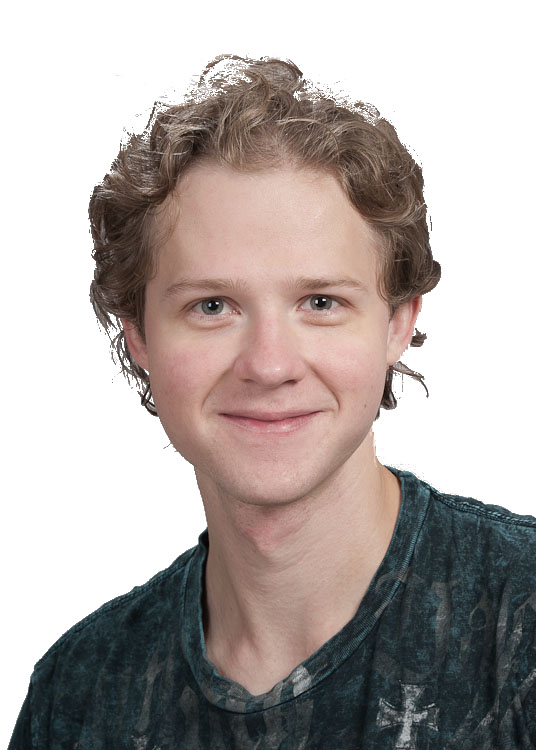
\includegraphics[width=1in,height=1.25in,clip,keepaspectratio]{photos/medley.jpg}}]{J. Kyle Medley}
obtained his BSc in Mechanical Engineering from the University of Missouri-Kansas City and
is currently pursuing a Ph.D. in Bioengineering from the University of Washington, USA.
His research interests include modeling dynamical biophysical processes such as
metabolism and gene expression regulation.
He currently develops libRoadRunner, a software package for simulating dynamical models encoded in SBML.
\end{IEEEbiography}

\begin{IEEEbiography}[{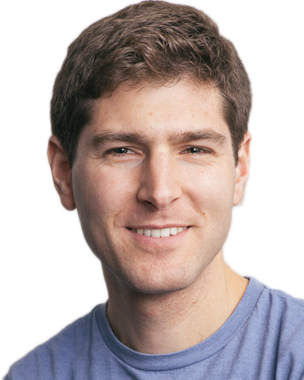
\includegraphics[width=1in,height=1.25in,clip,keepaspectratio]{photos/karr.jpg}}]{Jonathan R. Karr}
received his Ph.D. in Biophysics and M.S. in Medicine from Stanford University, USA in 2014 and his B.S.s in Physics and Brain \& Cognitive Sciences from the Massachusetts Institute of Technology, USA in 2006. Currently, Dr. Karr is a Fellow at the Icahn School of Medicine at Mount Sinai, USA. His research focuses on the development of comprehensive WC computational models and their application to bioengineering and medicine.
\end{IEEEbiography}

\vfill

\end{document}